\documentclass[tikz,border=12pt]{standalone}
\usepackage{amsmath,amssymb}
\usetikzlibrary{arrows.meta}

\begin{document}
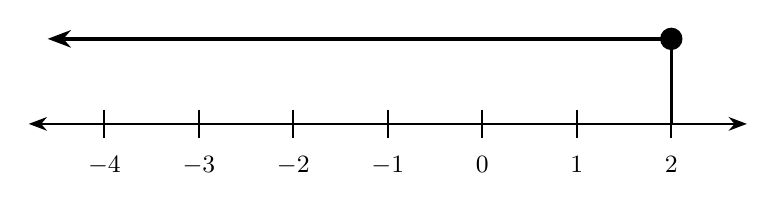
\begin{tikzpicture}[>=Stealth, scale=1.2]
    % Number line (adapted from diagram_01 template)
    % Mock item: closed dot at 2, ray to the left  =>  x <= 2
    \draw[thick, <->] (-4.8, 0) -- (2.8, 0);

    % Ticks and labels
    \foreach \x in {-4,-3,-2,-1,0,1,2} {
        \draw[thick] (\x, 0.15) -- (\x, -0.15) node[below=3pt, font=\small] {$\x$};
    }

    % Closed dot at 2 on a stem, arrow pointing left
    \draw[very thick] (2, 0) -- (2, 0.9);
    \filldraw[black] (2, 0.9) circle (3.2pt);
    \draw[very thick, ->] (2, 0.9) -- (-4.6, 0.9);
\end{tikzpicture}
\end{document}
